% Copyright 2014 Yoshida Shin
% 
% This is part of "Git Second Step."
% 
% This program is free software: you can redistribute it and/or modify
%     it under the terms of the GNU General Public License as published by
%     the Free Software Foundation, either version 3 of the License, or
%     (at your option) any later version.
% 
%     This program is distributed in the hope that it will be useful,
%     but WITHOUT ANY WARRANTY; without even the implied warranty of
%     MERCHANTABILITY or FITNESS FOR A PARTICULAR PURPOSE.  See the
%     GNU General Public License for more details.
% 
%     You should have received a copy of the GNU General Public License
%     along with this program.  If not, see <http://www.gnu.org/licenses/>.

\documentclass[dvipdfmx,slide,12pt]{beamer}
\usepackage{pxjahyper} % しおりの和文対応
\usetheme{PaloAlto} % テーマ名
\usepackage{minijs} % jsarticle のミニ版
\renewcommand{\kanjifamilydefault}{\gtdefault} % デフォルトフォントをゴシックに
\setbeamertemplate{navigation symbols}{} % dvipdfmx 対応
\usepackage{mymacro}

\title{git 次の一歩}

\begin{document}

\include{header}

\section{2種類の merge と rebase}
% Copyright 2014 Yoshida Shin
% 
% This is part of "Git Second Step."
% 
% This program is free software: you can redistribute it and/or modify
%     it under the terms of the GNU General Public License as published by
%     the Free Software Foundation, either version 3 of the License, or
%     (at your option) any later version.
% 
%     This program is distributed in the hope that it will be useful,
%     but WITHOUT ANY WARRANTY; without even the implied warranty of
%     MERCHANTABILITY or FITNESS FOR A PARTICULAR PURPOSE.  See the
%     GNU General Public License for more details.
% 
%     You should have received a copy of the GNU General Public License
%     along with this program.  If not, see <http://www.gnu.org/licenses/>.

\begin{frame}{}{}
  2種類の merge と rebase
\end{frame}

\begin{frame}[t]{2種類の merge}{}

  git の merge には

  ``first forward'' と ``no first forward''

  の2種類が存在
  \vspace{4ex}

  デフォルトではその時の branch の状況によって

  自動で使い分けられる
  \vspace{2ex}

  オプションを指定する事である程度制御可能
\end{frame}


\begin{frame}[t]{2種類の merge}{HEAD が merge 対象の先祖の時}

  \begin{columns}

    \begin{narrowcolumn}

      \begin{center}
        \begin{tikzpicture} [x=1em, y=1ex]

          \onslide<3->{\node (d4) [commit] at (4, 16) {A B};}
          \onslide*<1-2>{\node (d4) [commit] at (4, 16) {B};}
          \node (d3) [commit] at (4, 12) {};
          \onslide*<-2>{\node (m2) [commit] at (0, 8)  {A};}
          \onslide*<3->{\node (m2) [commit] at (0, 8)  {};}
          \node (m1) [commit] at (0, 4) {};
          \node (m0) [commit] at (0, 0) {};

          \draw (d3) -- (d4);
          \draw (m2) -- (d3);
          \draw (m1) -- (m2);
          \draw (m0) -- (m1);

        \end{tikzpicture}

        {\footnotesize{(A \alert{$\leftarrow$ HEAD})}}
      \end{center}

    \end{narrowcolumn}

    \begin{widecolumn}

      \onslide*<1>{
        A は B の先祖の commit
      }

      \onslide*<2-4>{
        \$ git merge B
        \vspace{2ex}

        \onslide*<4>{branch の向き先変更だけ}
      }

      \onslide*<5>{
        新しい commit が作られないので

        commit message の入力も無し
        \vspace{2ex}

        このように、

        新しい commit を作らない merge が

        first forward merge
      }

      \onslide*<6>{
        ちなみに、push では通常

        first forward merge を使用
      }
    \end{widecolumn}

  \end{columns}

\end{frame}


\begin{frame}[t]{2種類の merge}{HEAD が merge 対象が先祖では無い}

  \begin{columns}

    \begin{narrowcolumn}

      \begin{center}
        \begin{tikzpicture} [x=1em, y=1ex]

          \onslide<9->{\node (m7) [commit] at (0, 28) {A};}
          \onslide*<4-8>{\node (m7) [commit] at (0, 28) {}};

          \node (d6) [commit] at (4, 24) {B};
          \node (d5) [commit] at (4, 20) {};
          \node (d2) [commit] at (4, 8) {};

          \node (m4) [commit] at (0, 16) {\onslide*<-8>{A}};
          \node (m3) [commit] at (0, 12) {};
          \node (m1) [commit] at (0, 4) {};
          \node (m0) [commit] at (0, 0) {};

          \draw (d5) -- (d6);
          \draw (d2) -- (d5);
          \draw (m1) -- (d2);

          \draw (m3) -- (m4);
          \draw (m1) -- (m3);
          \draw (m0) -- (m1);

          \onslide*<6->{
            \draw [line width=2pt, color=green, ->] (m1) -- (m3) -- (m4);
            \draw [line width=2pt, color=green, ->] (d6) -- (m7);
          }
          \onslide*<4->{
            \draw [line width=2pt, color=red, ->] (m4) -- (m7);
          }
          \onslide*<3->{
            \draw [line width=2pt, color=red, ->] (m1) -- (d2) -- (d5) -- (d6);
          }
        \end{tikzpicture}

        {\footnotesize{(A \alert{$\leftarrow$ HEAD})}}
      \end{center}

    \end{narrowcolumn}

    \begin{widecolumn}

      \onslide*<1>{
        A と B は branch の分岐後

        それぞれ開発
      }

      \onslide*<2-4>{
        \$ git merge B
        \vspace{2ex}

        \onslide*<3-4>{
          B の更新分のパッチを

          A に適用し、

          新しい commit object を作成}
      }

      \onslide*<5-6>{
        衝突が無ければ、A のパッチを

        B に適用しても同じ物になるはず
      }

      \onslide*<7>{
        新しい commit を作るので

        commit message を入力
      }

      \onslide*<8-9>{
        HEAD を新しい commit へ移動
      }

      \onslide*<10>{
        このように、

        新しい commit が作られる merge が

        no first forward merge
      }
    \end{widecolumn}

  \end{columns}

\end{frame}


\begin{frame}[t]{2種類の merge}{commit tree が 2又の時}

  \begin{columns}

    \begin{narrowcolumn}

      \begin{center}
        \begin{tikzpicture} [x=1em, y=1ex]

          \node (m7) [commit] at (0, 28) {A};

          \node (d6) [commit] at (4, 24) {B};
          \node (d5) [commit] at (4, 20) {};
          \node (d2) [commit] at (4, 8) {};

          \node (m4) [commit] at (0, 16) {};
          \node (m3) [commit] at (0, 12) {};
          \onslide*<4-6>{\node (m3) [commit] at (0, 12) {\alert{?}};}
          \node (m1) [commit] at (0, 4) {};
          \node (m0) [commit] at (0, 0) {};


          \onslide*<1,8->{
            \draw (d6) -- (m7);
            \draw (d5) -- (d6);
            \draw (d2) -- (d5);
            \draw (m1) -- (d2);

            \draw (m4) -- (m7);
            \draw (m3) -- (m4);
            \draw (m1) -- (m3);
            \draw (m0) -- (m1);
          }

          \onslide*<2-7>{
            \draw (d6) -- (m7);
            \draw (d5) -- (d6);
            \draw (m4) -- (d5);
            \draw (m3) -- (m4);
            \draw (d2) -- (m3);
            \draw (m1) -- (d2);
            \draw (m0) -- (m1);
          }
        \end{tikzpicture}
      \end{center}

    \end{narrowcolumn}

    \begin{widecolumn}
      \onslide*<1-2>{
        ちなみに、オプション無しで

        \$ git log A

        を実行すると、
      }

      \onslide*<3>{こう勘違いするかも}

      \onslide*<4-5>{
        例えばここ、
        \vspace{2ex}

        どうなってるの?
        \vspace{4ex}

        \onslide*<5>{
          B の 1個目の commit と

          A の 1個目の commit が

          merge されて......
          \vspace{4ex}

          あれ、衝突は?
        }
      }

      \onslide*<6>{どうもなっていません!}

      \onslide*<7->{
        あくまでも、正しいのはこっち
        \vspace{2ex}

        \onslide*<9->{
          \$ git log {\dhyphen}graph A
          \vspace{2ex}

          で確認可能
        }
        \vspace{2ex}

        \onslide*<10->{
          merge による変化は、

          commit 1個追加のみ
        }
        \vspace{2ex}

        \onslide*<11>{
          既存の commit は

          変化無し
        }
      }
    \end{widecolumn}
  \end{columns}
\end{frame}


\begin{frame}[t]{2種類の merge}{HEAD が merge 対象の先祖の時}

  \begin{columns}

    \begin{narrowcolumn}

      \begin{center}
        \begin{tikzpicture} [x=1em, y=1ex]

          \onslide<5->{\node (m5) [commit] at (0, 20) {A};}
          \onslide<3>{\node (d4) [commit] at (4, 16) {A B};}
          \onslide*<1-2,4->{\node (d4) [commit] at (4, 16) {B};}
          \node (d3) [commit] at (4, 12) {};
          \node (m2) [commit] at (0, 8)  {\onslide*<-2,4>{A}};
          \node (m1) [commit] at (0, 4) {};
          \node (m0) [commit] at (0, 0) {};


          \onslide*<5->{
            \draw (d4) -- (m5);
            \draw (m2) -- (m5);
          }
          \draw (d3) -- (d4);
          \draw (m2) -- (d3);
          \draw (m1) -- (m2);
          \draw (m0) -- (m1);

        \end{tikzpicture}

        {\footnotesize{(A \alert{$\leftarrow$ HEAD})}}
      \end{center}

    \end{narrowcolumn}

    \begin{widecolumn}
      \onslide*<1>{
        A が B の先祖の場合
        \vspace{4ex}

        merge コマンドに

        オプションを付与して

        merge 方法を選択可能
      }

      \onslide*<2-3>{
        {\dhyphen}ff-only オプションで

        first forward を強制
        \vspace{2ex}

        \$ git merge B {\dhyphen}ff-only
        \vspace{2ex}

        first forward できない場合に

        エラーになる
      }

      \onslide*<4-5>{
        {\dhyphen}no-ff オプションで

        no first foward を強制
        \vspace{2ex}

        \$ git merge {\dhyphen}no-ff B
        \vspace{2ex}

        HEAD が merge 対象の先祖でも

        無理矢理 no first forward で

        merge する
      }

      \onslide*<6>{
        デフォルトオプションは {\dhyphen}ff
        \vspace{2ex}

        可能であれば first forward,

        無理ならば no first forward
        \vspace{2ex}

        という意味
      }

    \end{widecolumn}

  \end{columns}

\end{frame}


\begin{frame}[t]{merge の種類とオプションまとめ}{}

  \begin{table}[htb]

    \begin{tabular}{c|ccc}
      \shortstack{\footnotesize HEAD が \\ \footnotesize 対象の} & {\small {\dhyphen}ff-only} & {\small {\dhyphen}ff (デフォルト)} & {\small {\dhyphen}no-ff} \\ \hline
      先祖 & {\small first forward} & {\small first forward} & {\small no first forward} \\
      & & & \\
      \shortstack{\footnotesize 先祖 \\ \footnotesize ではない} & エラー & {\small no first forward} & {\small no first forward}
    \end{tabular}
  \end{table}

\end{frame}


\begin{frame}[t]{2種類の merge の特徴}{first forward merge}
  first forward merge
  \vspace{2ex}

  \begin{itemize}
  \item 衝突等 merge に伴う事故が最も少ない
    \vspace{2ex}

  \item {\dhyphen}ff-only オプションで安全性の担保も可能
    \vspace{2ex}

  \item 過去の履歴が一直線なので簡単
  \end{itemize}
  \vspace{2ex}
\end{frame}


\begin{frame}[t]{2種類の merge の特徴}{no first forward merge}
  no first forward merge
  \vspace{2ex}

  \begin{itemize}
  \item branch だけで色々と主張できる
    \begin{itemize}
    \item 別 branch の複数の commit は関連する
    \item 別 branch の commit を 1個だけ適用すると

      中途半端な状況になる
    \end{itemize}
    \vspace{2ex}

  \item 過去の経緯が複雑
    \vspace{2ex}

  \item 親が複数有るので、パッチや履歴対象の操作が難しくなる\footnote{この欠点については今回の範囲を超えるので省略}
  \end{itemize}
\end{frame}


\begin{frame}[t]{merge の問題点}{}
  HEAD が merge 対象の先祖の場合は大きな問題は無い

  first forward と no first forward の好きな方を選べば良い
  \vspace{2ex}

  問題はそれ以外の場合

  \onslide<2->{特に、remote repository から更新を取り入れる時}
  \vspace{2ex}

  \onslide<3->{
    \begin{itemize}
    \item 「更新と取り込むため」だけの

      無意味な branch, commit が出来る

      (履歴を追う際のノイズになる)
      \onslide<4->{\item 複数 branch 間の merge は履歴が複雑}
    \end{itemize}
  }

  \onslide<5->{履歴を追えなければ SCM の意味が無い}
\end{frame}

% Copyright 2014 Yoshida Shin
% 
% This is part of "Git Second Step."
% 
% This program is free software: you can redistribute it and/or modify
%     it under the terms of the GNU General Public License as published by
%     the Free Software Foundation, either version 3 of the License, or
%     (at your option) any later version.
% 
%     This program is distributed in the hope that it will be useful,
%     but WITHOUT ANY WARRANTY; without even the implied warranty of
%     MERCHANTABILITY or FITNESS FOR A PARTICULAR PURPOSE.  See the
%     GNU General Public License for more details.
% 
%     You should have received a copy of the GNU General Public License
%     along with this program.  If not, see <http://www.gnu.org/licenses/>.

\begin{frame}[t]{first forward merge できない場合}{}

  \begin{columns}

    \begin{narrowcolumn}

      \begin{center}
        \begin{tikzpicture} [x=1em, y=1ex]

          \onslide<11-13,16->{
            \node (d11) [commit] at (4, 22) {A};
            \node (d9) [commit] at (4, 18) {};
          }

          \onslide*<2-5>{\node (m8) [commit] at (0, 16) {A};}

          \onslide*<9-10>{\node (d7) [commit] at (4, 14) {A B};}
          \onslide*<1-8,11->{\node (d7) [commit] at (4, 14) {B};}
          \node (d5) [commit] at (4, 10) {};
          \node (d3) [commit] at (4, 6) {};

          \onslide*<2-5,9-13,16->{\node (m6) [commit] at (0, 12) {};}
          \onslide*<1,6-8,14-15>{\node (m6) [commit] at (0, 12) {A};}
          \node (m4) [commit] at (0, 8) {};
          \node (m2) [commit] at (0, 4) {};
          \node (m0) [commit] at (0, 0) {};

          \onslide*<11-13,16->{
            \draw [line width=3pt, color = red] (d9) -- (d11);
            \draw [line width=3pt, color = green] (d7) -- (d9);
          }

          \onslide*<7-13,16->{
            \draw [line width=3pt, color = red] (m4) -- (m6);
            \draw [line width=3pt, color = green] (m2) -- (m4);
          }

          \onslide*<2-5>{
            \draw (d7) -- (m8);
            \draw (m6) -- (m8);
          }

          \draw (d5) -- (d7);
          \draw (d3) -- (d5);
          \draw (m2) -- (d3);

          \onslide*<-6,14-15>{
            \draw (m4) -- (m6);
            \draw (m2) -- (m4);
          }
          \draw (m0) -- (m2);

        \end{tikzpicture}

        {\footnotesize{(A \alert{$\leftarrow$ HEAD})}}
      \end{center}

    \end{narrowcolumn}

    \begin{widecolumn}

      \onslide*<1-5>{
        方法1

        気にせず no first forward merge

        \onslide<3->{
          \begin{itemize}
          \item 簡単に実行可能
            \onslide<4->{
            \item よーく考えると

              \onslide<5>{全然解決になっていない}
            }
          \end{itemize}
        }
      }

      \onslide*<6-13>{
        方法2

        git diff により A 上の

        commit のパッチを作成
        \vspace{2ex}

        \onslide*<8->{A の向き先を B へ変更}
        \vspace{2ex}

        \onslide<10->{
          作ったパッチを適用し、

          新しく commit
        }

        \onslide<12->{
          \begin{itemize}
          \item 履歴が 1直線になる
            \onslide<13->{\item パッチ適用の数だけ衝突の可能性あり}
            \onslide<14->{\item 手作業が辛い}
          \end{itemize}
        }
      }

      \onslide*<14-18>{
        方法3

        方法2 を自動化する

        \onslide<15->{\$ git rebase A}

        \onslide<17->{
          \begin{itemize}
          \item 履歴が 1直線になる
            \onslide<18->{\item commit の数だけ衝突する可能性あり}
          \end{itemize}
        }
      }

      \onslide*<19->{
        図から分かるように、rebase により

        commit が消える事は無い
        \vspace{2ex}

        \onslide*<20->{branch から外れるだけ}
        \vspace{2ex}

        \onslide*<21->{
          gc の前ならば、切り戻し可能

          (デフォルトの gc では、数日間は消されない)
        }
        \vspace{2ex}

        \onslide*<22->{
          rebase に限らず、git では一般的に

          commit がその場で消える事は無い

          多くの場合、切り戻し可能
        }
      }
    \end{widecolumn}
  \end{columns}

\end{frame}


\section{過去の履歴を書き換える}
% Copyright 2014 Yoshida Shin
% 
% This is part of "Git Second Step."
% 
% This program is free software: you can redistribute it and/or modify
%     it under the terms of the GNU General Public License as published by
%     the Free Software Foundation, either version 3 of the License, or
%     (at your option) any later version.
% 
%     This program is distributed in the hope that it will be useful,
%     but WITHOUT ANY WARRANTY; without even the implied warranty of
%     MERCHANTABILITY or FITNESS FOR A PARTICULAR PURPOSE.  See the
%     GNU General Public License for more details.
% 
%     You should have received a copy of the GNU General Public License
%     along with this program.  If not, see <http://www.gnu.org/licenses/>.

\begin{frame}{}{}
  過去の履歴を書き換える
\end{frame}


\begin{frame}[t]{過去の履歴を書き換える}{}
  SCM の悪い履歴とは?

  \onslide*<2->{
    \begin{itemize}
    \item 紆余曲折がそのままでノイズ多
      \begin{enumerate}
      \item method A, B, C を実装
      \item method B のバグ修正
      \item 結局、method A, B は削除
      \end{enumerate}
      \onslide*<3->{最初から method C だけ書いてよ}
      \vspace{2ex}

      \onslide*<4->{
      \item 動作確認出来ない的 commit

        (括弧の閉じ忘れで動かない等)
      }

    \end{itemize}
  }
\end{frame}


\begin{frame}[t]{過去の履歴を書き換える}{}
  悪い履歴を残さないためには?
  \vspace{4ex}

  \onslide*<2->{
    commit の度にしっかりテスト、吟味する
    \onslide*<3->{
      \begin{enumerate}
      \item 副作用として、commit のハードルが上がる
        \onslide*<4->{\item 大きい commit を少数行うようになる}
        \onslide*<5->{
        \item 突き詰めると、commit 1個 だけ(完成品のみ)

          に行き着く

          super water fall 万歳
        }
      \end{enumerate}
    }
  }
  \vspace{4ex}

  \onslide*<6->{少し大げさかもしれないが、何かおかしくない?}
\end{frame}


\begin{frame}[t]{過去の履歴を書き換える}{}
  悪い履歴を残さない、もう一つの方法は

  過去の履歴の修正
  \vspace{4ex}

  \onslide*<2->{
    \begin{itemize}
    \item 古い commit のバグが、後になって発覚

      \onslide*<3->{バグ修正 commit の追加より、古い commit の修正}
      \vspace{2ex}

      \onslide*<4->{
      \item 最終的に、特定の commit が不要になった

        \onslide*<5->{
          不要部分の削除 commit より、

          該当箇所を実装した commit 自体の削除
        }
      }
    \end{itemize}
  }
  \vspace{4ex}

  \onslide*<6->{
    git なら、履歴の修正が可能

    最終的に悪い履歴が残らなければ良い
  }
\end{frame}


\begin{frame}[t]{過去の履歴を書き換える}{}
  ただし、履歴を修正してはいけない branch も有る
  \vspace{2ex}

  修正して良い例
  \begin{itemize}
  \item local repository の branch
  \item クローズドな repository 内で

    閲覧、更新者が限られた branch
    \begin{itemize}
    \item レビューのため、個人名をつけた branch
    \item 担当者のアサインされた topic branch
    \end{itemize}
  \end{itemize}
  \vspace{2ex}

  修正してはいけない例
  \begin{itemize}
  \item 不特定多数の人が閲覧可能な branch
  \item その他、一般的な remote reposiotry の branch
  \end{itemize}
\end{frame}


\begin{frame}[t]{過去の履歴を書き換える}{}
  SCM の履歴はドキュメンタリーでは無い

  不要な物は捨てて、必要十分な情報のみ残す
  \vspace{2ex}

  しかし、失敗を恐れて commit を控えれば、

  SCM の機能を十分に使わない事になる
  \vspace{4ex}

  要するに、最終的に複数人で共有する branch へ

  push する時までに直せば良い

  それまでは気軽に commit するべき

\end{frame}


\begin{frame}[t]{過去の履歴を書き換える}{}

  \begin{columns}

    \begin{narrowcolumn}

      \begin{center}
        \begin{tikzpicture}[x=1em, y=1ex]

          \node (G) [commit] at (0, 24) {G};
          \node (F) [commit] at (0, 20) {F};
          \node (E) [commit] at (0, 16) {E};
          \node (D) [commit] at (0, 12) {D};
          \node (C) [commit] at (0, 8) {C};
          \node (B) [commit] at (0, 4) {B};
          \node (A) [commit] at (0, 0) {A};

          \draw (F) -- (G);
          \draw (E) -- (F);
          \draw (D) -- (E);
          \draw (C) -- (D);
          \draw (B) -- (C);
          \draw (A) -- (B);

        \end{tikzpicture}

        {\footnotesize{(G \alert{$\leftarrow$ HEAD})}}
      \end{center}

    \end{narrowcolumn}

    \begin{widecolumn}

      直近 6個の履歴 (B, C, D, E, F, G) を見直す場合
      \vspace{2ex}

      \$ git rebase -i \textit{A}
      \vspace{2ex}

      を実行
      \vspace{2ex}

      (B の1個前の commit を指定する)

      (commit の指定方法は branch, tag, ハッシュ値等)
    \end{widecolumn}

  \end{columns}

\end{frame}


\begin{frame}[t]{過去の履歴を書き換える}{}

  \begin{columns}

    \begin{halfcolumn}
      \code{\onslide*<-4>{\alert<2>{pick}}\onslide*<5->{\alert{r}}~824c7c9~message~B

        \alert<2>{pick}~36dc484~message~C

        \onslide*<-6>{\alert<2>{pick}}\onslide*<7->{\alert{f}}~9a7c30a~message~D

        \onslide*<9->{\alert{\#}}\alert<2>{pick}~0ed3c2e~message~E

        \onslide*<-10>{
          \alert<2>{pick}~b7a1a35~message~F

          \alert<2>{pick}~ac859a3~message~G
        }

        \onslide*<11->{
          \alert{f}~ac859a3~message~G

          pick~b7a1a35~message~F
        }

        ...
      }

    \end{halfcolumn}

    \begin{halfcolumn}

      \onslide*<1>{
        エディタが開き、

        左のような画面が表示
        \vspace{2ex}

        上が古く、下が新しい

        (git log と逆なので注意)
      }

      \onslide*<2>{
        この画面では、

        どの履歴を編集するか指定
        \vspace{4ex}

        実際に履歴を編集するのは後
        \vspace{2ex}

        書き換えるのは主に\alert{この列}
      }

      \onslide*<3>{
        ``pick'' は「何も手を加えない」という意味
      }

      \onslide*<4-5>{
        B の commit message を

        変更するには
        \vspace{4ex}

        B の ``pick'' を ``r'' に変更

        (または、``reword'' に変更)
      }

      \onslide*<6-7>{
        D の commit を

        前の commit (C) と

        1個にまとめるには
        \vspace{4ex}

        D の ``pick'' を ``f''に変更

        (または、``fixup'' に変更)
      }

      \onslide*<8-9>{
        E の commit を削除するには

        E の行をコメントアウト
        \vspace{2ex}

        (履歴を残さない事以外は

        git revert と似ている)
      }

      \onslide*<10-11>{
        G の commit を
        前の commit (C+D) と

        1個にまとめるには
        \vspace{4ex}

        F と G の行を入れ替えて

        G の ``pick'' を ``f'' に変更する
      }

      \onslide*<12>{
        この状態でエディタを

        保存、終了
      }

    \end{halfcolumn}

  \end{columns}

\end{frame}

\begin{frame}[t]{過去の履歴を書き換える}{}
  \begin{columns}

    \begin{halfcolumn}

      \begin{center}
        \begin{tikzpicture}[x=1em, y=1ex]

          \node (G) [commit] at (0, 24) {G};
          \node (F) [commit] at (0, 20) {F};
          \node (E) [commit] at (0, 16) {E};
          \node (D) [commit] at (0, 12) {D};
          \node (C) [commit] at (0, 8) {C};
          \node (B) [commit] at (0, 4) {B};
          \node (A) [commit] at (0, 0) {A};

          \onslide*<-7>{
            \draw (E) -- (F);
          }

          \draw (D) -- (E);

          \onslide*<-5>{
            \draw (F) -- (G);
            \draw (C) -- (D);
            \draw (B) -- (C);
          }
          \onslide*<-3>{\draw (A) -- (B);}


          \onslide<8->{\node (F') [commit] at (6, 20) {F'};}
          \onslide<6->{\node (C') [commit] at (6, 16) {C+D+G};}
          \onslide<4->{\node (B') [commit] at (6, 4) {B'};}

          \onslide*<8->{
            \draw [line width=3pt, color=blue] (E) -- (F);
            \draw [line width=3pt, color=blue] (C') -- (F');
          }

          \onslide*<6->{
            \draw [line width=3pt, color=green] (B') -- (C');
            \draw [line width=3pt, color=green] (F) -- (G);
            \draw [line width=3pt, color=green] (C) -- (D);
            \draw [line width=3pt, color=green] (B) -- (C);
          }

          \onslide*<4->{
            \draw [line width=3pt, color=red] (A) -- (B');
            \draw [line width=3pt, color=red] (A) -- (B);
          }
        \end{tikzpicture}
      \end{center}

    \end{halfcolumn}

    \begin{halfcolumn}

      \onslide*<1>{
        まず、HEAD を A に切り替える
      }

      \onslide*<2>{
        エディタが開き、

        B の commit message

        再入力
      }

      \onslide*<3-4>{
        B のパッチを

        A に適用
      }

      \onslide*<5-6>{
        C+D+G のパッチを

        B' へ適用
        \vspace{4ex}

        Commit message は

        C の物を使用
      }

      \onslide*<7-8>{
        F は pick なので、

        何もせず F のパッチを

        C+D+G に適用
      }


      \onslide*<9-10>{
        その他、

        r と f を一度に実行する

        s (または squash)
        \vspace{2ex}

        \onslide*<10>{
          rebase を一回止める

          e (または edit)

          (この間に色々出来る)
          \vspace{2ex}

          もある
        }
      }

      \onslide*<11->{
        でも、個人的には

        s や e が役に立った

        記憶が少ないので

        説明省略
      }
      \vspace{2ex}

      \onslide*<12->{気になる人は、man で調べて}

    \end{halfcolumn}

  \end{columns}

\end{frame}


\begin{frame}[t]{過去の履歴を書き換える}{}

  ところで、
  \vspace{2ex}

  \onslide*<2->{
    初めから fixup する予定で commit したのなら

    commit message に更新内容を書く必要は無い

    どの commit に fixup する予定かを示せば十分
  }
  \vspace{2ex}

  \onslide*<3->{
    \$ git commit {\dhyphen}fixup=\textit{commit}

    とすると、
    \vspace{2ex}

    ``fixup! {\textless}\textit{commit} の message\textgreater''

    という commit message をつけて commit してくれる
  }
  \vspace{2ex}

  \onslide*<4->{
    同様の

    \$ git commit {\dhyphen}squash=\textit{commit}

    というコマンドもある
  }
  \vspace{2ex}

\end{frame}


\begin{frame}[t]{過去の履歴を書き換える}{}
  個人的には、commit の指定には

  圧倒的に HEAD が多い
  \vspace{4ex}

  git commit {\dhyphen}fixup=HEAD

  や

  git commit {\dhyphen}squash=HEAD
  \vspace{2ex}

  は長いので、alias を張ってます
\end{frame}


\begin{frame}[t]{過去の履歴を書き換える}{}
  \$ git config {\dhyphen}global alias.fixup {\bslash}

  ~~~~``commit {\dhyphen}fixup=HEAD''

  \$ git config {\dhyphen}global alias.squash {\bslash}

  ~~~~``commit {\dhyphen}squash=HEAD''
  \vspace{2ex}

  \onslide*<2->{
    こうすると、

    \$ git fixup (\$ git squash)

    と実行するだけで
    \vspace{2ex}

    git commit {\dhyphen}fixup=HEAD

    (git commit {\dhyphen}squash=HEAD)
    \vspace{2ex}

    と同じ意味になる
  }
\end{frame}


\begin{frame}[t]{過去の履歴を書き換える}{}

  さらに言うと、
  \vspace{2ex}

  \onslide*<2->{
    commit message に fixup や squash の印が

    フォーマットに従って記載してあれば、

    rebase -i する時に f や s の印をつける事を

    機械的に判断可能
  }
  \vspace{2ex}

  \onslide*<3->{じゃあ、機械にやってもらいましょう}

\end{frame}


\begin{frame}[t]{過去の履歴を書き換える}{}
  \$ git rebase -i \textit{commit} {\dhyphen}autosquash
  \vspace{4ex}


  先頭が fixup! や squash! で始まり

  続く commit message が commit 再編集の対象の場合
  \vspace{2ex}


  commit message に従って

  fixup や squash の印をつけ、

  commit の順番入れ替えまで実行済みの状態で

  rebase -i のエディタが開く
\end{frame}


\begin{frame}[t]{過去の履歴を書き換える}{}
  \$ git rebase -i \textit{commit} {\dhyphen}autosquash
  \vspace{2ex}

  も長い?
  \vspace{4ex}

  \onslide*<2>{
    \$ git config {\dhyphen}global rebase.autosquash true
    \vspace{2ex}

    とすると、

    rebase -i 時に毎回 {\dhyphen}autosquash をデフォルトでつけてくれる
  }
\end{frame}


\begin{frame}[t]{過去の履歴を書き換える}{}

  良く言われるように、git は branch 作成コストが低く

  master に影響を与える事なく、実験が出来る
  \vspace{2ex}

  \onslide*<2->{
    実験の結果、うまくいった commit を取り込み、

    不要な commit を外すのにも rebase -i は便利
    \vspace{2ex}

    \onslide<3->{フィードバックを行うまでが実験!}
  }
  \vspace{2ex}

  \onslide*<4->{
    個人的には、push しない事前提に

    デバッグ用のコード (print 文等) を仕込んだ

    commit も好き
  }
\end{frame}


\section{merge と rebase の使用方法例}
% Copyright 2014 Yoshida Shin
% 
% This is part of "Git Second Step."
% 
% This program is free software: you can redistribute it and/or modify
%     it under the terms of the GNU General Public License as published by
%     the Free Software Foundation, either version 3 of the License, or
%     (at your option) any later version.
% 
%     This program is distributed in the hope that it will be useful,
%     but WITHOUT ANY WARRANTY; without even the implied warranty of
%     MERCHANTABILITY or FITNESS FOR A PARTICULAR PURPOSE.  See the
%     GNU General Public License for more details.
% 
%     You should have received a copy of the GNU General Public License
%     along with this program.  If not, see <http://www.gnu.org/licenses/>.

\begin{frame}{}{}
  merge と rebase の使用方法例
\end{frame}

\begin{frame}[t]{branch 輪廻から解脱}{}
  \begin{center}
    \begin{tikzpicture} [x=1em, y=1ex]
      \onslide<17->{\node (3) [commit] at (8,20) {master};}

      \onslide<9->{
        \onslide<13-14>{\node (E) [commit] at (16,16) {master devel};}
        \onslide*<15->{\node (E) [commit] at (16,16) {devel};}
        \onslide*<-12>{\node (E) [commit] at (16,16) {master};}
        \node (D) [commit] at (16,12) {};
      }

      \onslide<15-16>{
        \node (2) [commit, rectangle split, rectangle split parts=2] at (8,8){
          {master}
          \nodepart{second}{\tiny remotes/origin/master}
        };
      }
      \onslide*<7-14,17->{\node (2) [commit] at (8,8) {remotes/origin/master};}
      \onslide*<7->{\node (1) [commit] at (8,4) {};}

      \onslide*<3-4>{\node (D) [commit] at (0,12) {master};}

      \onslide*<3-8>{
        \node (C) [commit] at (0,8) {\onslide*<5->{master}};
        \node (B) [commit] at (0,4) {};
      }

      \onslide<-2>{\node (A) [commit] at (0,0) {master};}
      \onslide*<3->{\node (A) [commit] at (0,0) {};}

      \onslide*<17->{
        \draw (E) -- (3);
        \draw (2) -- (3);
      }

      \onslide*<9->{
        \draw (D) -- (E);
        \draw (2) -- (D);
      }

      \onslide*<7->{
        \draw (1) -- (2);
        \draw (A) -- (1);
      }

      \onslide*<3-4>{\draw (C) -- (D);}

      \onslide*<3-8>{
        \draw (B) -- (C);
        \draw (A) -- (B);
      }
    \end{tikzpicture}
  \end{center}

  \onslide*<1>{
    remote から clone したレポジトリで

    他の人と共同開発する場合
  }

  \onslide*<2-3>{
    master で開発開始
  }

  \onslide*<4-5>{
    master の履歴を整理
    \vspace{4ex}

    \$ git rebase -i ***
  }

  \onslide*<6-7>{
    remote branch をアップデート

    \$ git fetch {\dhyphen}all -p
  }

  \onslide*<8-9>{
    remote branch の更新を master に反映

    \$ git rebase remotes/origin/master
  }

  \onslide*<10>{
    commit tree を 1本にしたい場合は

    これで終了
  }

  \onslide*<11>{
    github で pull request 出す時は、

    この状態で出すと良い
  }

  \onslide*<12-13>{
    commit tree を 2本にする場合は

    現在の HEAD に適当な新しいブランチ作成

    \$ git branch devel
  }

  \onslide*<14-15>{
    HEAD を remote branch の最新状態まで

    巻き戻す

    \$ git reset remotes/origin/master
  }

  \onslide*<16-17>{
    devel を no first forward で merge

    \$ git merge devel {\dhyphen}no-ff
  }

\end{frame}


\begin{frame}[t]{branch 輪廻から解脱}{}

  ところで

  「no first forward の merge をする場合は

   rebase 必要ないのでは?」

  と思った人
  \vspace{4ex}

  \onslide<2->{\alert{鋭い}}
  \vspace{4ex}

  \onslide<3->{
    と見せて

    \alert{あまい}
  }

\end{frame}


\begin{frame}<1-13>[t]{branch 輪廻から解脱}{}

  自分が作業している間に remote branch が更新されたら

  \begin{columns}

    \begin{narrowcolumn}
      \begin{center}
        \begin{tikzpicture} [x=1em, y=1ex]

          \onslide<99>{\node (dummy) [commit] at (0, 16) {};}

          \onslide<3->{\node (C) [commit] at (0, 12) {};}

          \node (2) [commit] at (3,8) {};
          \node (1) [commit] at (3,4) {};
          \node (B) [commit] at (0,4) {};
          \node (A) [commit] at (0,0) {};

          \onslide<3->{
            \draw (2) -- (C);
            \draw (B) -- (C);
          }

          \draw (1) -- (2);
          \draw (A) -- (1);
          \draw (A) -- (B);
        \end{tikzpicture}

        merge のみ
      \end{center}
    \end{narrowcolumn}

    \begin{narrowcolumn}
      \begin{center}
        \begin{tikzpicture} [x=1em, y=1ex]

          \onslide<99>{\node (dummy) [commit] at (0, 16) {};}

          \onslide<7->{
            \node (2) [commit] at (3,12) {};
            \node (1) [commit] at (3,8) {};
          }

          \onslide*<-6>{
            \node (2) [commit] at (3,8) {};
            \node (1) [commit] at (3,4) {};
          }
          \node (B) [commit] at (0,4) {};
          \node (A) [commit] at (0,0) {};

          \onslide<7->{\draw (B) -- (1);}
          \draw (1) -- (2);
          \onslide<-6>{\draw (A) -- (1);}
          \draw (A) -- (B);
        \end{tikzpicture}

        rebase のみ
      \end{center}
    \end{narrowcolumn}

    \begin{narrowcolumn}
      \begin{center}
        \begin{tikzpicture} [x=1em, y=1ex]
          \onslide<10->{
            \node (C) [commit] at (0,16) {};
            \node (2) [commit] at (3,12) {};
            \node (1) [commit] at (3,8) {};
          }

          \onslide*<-9>{
            \node (2) [commit] at (3,8) {};
            \node (1) [commit] at (3,4) {};
          }
          \node (B) [commit] at (0,4) {};
          \node (A) [commit] at (0,0) {};

          \onslide<10->{
            \draw (2) -- (C);
            \draw (B) -- (C);
            \draw (B) -- (1);
          }
          \draw (1) -- (2);
          \onslide<-9>{\draw (A) -- (1);}
          \draw (A) -- (B);
        \end{tikzpicture}

        rebase + merge
      \end{center}
    \end{narrowcolumn}

  \end{columns}
  \vspace{2ex}

  \onslide*<2>{rebase せずに merge で取り込む}

  \onslide*<4-5>{
    \alert{今回は} branch が 2又に分かれる

    \onslide*<5>{
      より正確には、開発ラインの数 (= 開発者の数?)だけ

      branch が分かれ、merge が入り乱れる
    }
  }

  \onslide*<6>{rebase で取り込む}

  \onslide*<8>{開発ラインの数によらず、branch は 1本}

  \onslide*<9>{rebase してから no first forward merge で取り込む}

  \onslide*<11>{
    開発ラインの数によらず、

    更新の有る branch は常に 1本
  }


  \onslide*<12>{
    その他、更新の無い branch が最大 1本

    branch が合計 3本以上になる事は無い
  }

  \onslide*<13>{
    結論

    branch のアミダクジ状態を避ける為には

    rebase は必要
  }
\end{frame}


\section{今更 git pull}
% Copyright 2014 Yoshida Shin
% 
% This is part of "Git Second Step."
% 
% This program is free software: you can redistribute it and/or modify
%     it under the terms of the GNU General Public License as published by
%     the Free Software Foundation, either version 3 of the License, or
%     (at your option) any later version.
% 
%     This program is distributed in the hope that it will be useful,
%     but WITHOUT ANY WARRANTY; without even the implied warranty of
%     MERCHANTABILITY or FITNESS FOR A PARTICULAR PURPOSE.  See the
%     GNU General Public License for more details.
% 
%     You should have received a copy of the GNU General Public License
%     along with this program.  If not, see <http://www.gnu.org/licenses/>.

\begin{frame}{}{}
  今更 git pull
\end{frame}


\begin{frame}[t]{今更 git pull}{}
  ネットでは

  「git を良く知らない間は pull はやめた方が良い」

  と良く言われる
  \vspace{4ex}

  \onslide*<2>{
    その割には、

    良く知っている人はどうやって使うのか

    あまり記載が無いので、私なりの回答をご紹介
  }

  \onslide*<3->{なぜやめた方が良いのか?}
  \vspace{4ex}

  \onslide*<4->{
    git pull はリモートブランチの更新を取り込む

    shell script
  }
  \vspace{2ex}

  \onslide*<5->{デフォルトの挙動は、fetch + merge}
  \vspace{2ex}

  \onslide*<6->{merge のアンチパターン直撃}
\end{frame}


\begin{frame}[t]{今更 git pull}{}
  git pull との上手な接し方
  \onslide*<2->{
    \begin{enumerate}
    \item 使わない
      \onslide*<3->{\item 挙動を fetch + rebase に変更}
      \onslide*<4->{\item no first forward merge を禁止}
    \end{enumerate}
  }
\end{frame}


\begin{frame}[t]{今更 git pull}{}
  git pull 使わない
  \vspace{2ex}

  \begin{itemize}
  \item fetch + rebase で十分
  \item remote の更新確認は頻繁に行う

    しかし、更新取り込みは別のタイミングで行いたい

    更新確認の度に衝突の危機になったり、

    自分のコードが変更されるるのは非生産的

    思考を中断しない為に、結局 fetch を使う
  \end{itemize}
  \vspace{2ex}

  \onslide*<2>{私は、普段この方法}
\end{frame}


\begin{frame}[t]{今更 git pull}{}
  挙動を fetch + rebase にする
  \vspace{2ex}

  \onslide*<1->{
    \begin{itemize}
    \item 手軽に remote の更新を local に反映できる
    \item 衝突が発生しやすい
    \end{itemize}
  }
  \vspace{2ex}

  \onslide*<2->{
    設定方法

    \$ git config {\dhyphen}global pull.rebase true
  }
  \vspace{2ex}

  \onslide*<3>{簡単な開発の場合は、私はこの方法を使います}
\end{frame}


\begin{frame}[t]{今更 git pull}{}
  no first forward merge を禁止
  \vspace{2ex}

  \onslide*<1->{
    \begin{itemize}
    \item local での開発には開発用 branch で行う必要あり
    \item pull に限らず、no first foward を禁止すると

      merge に関わる事故や問題の多くを回避可能

      うっかりミス防止のため、システム的に禁止
    \item no first forward merge は、有るから使う程度

      個人的には、無くても大きな問題は無い気がする
    \end{itemize}
  }
  \vspace{2ex}

  \onslide*<2->{
    設定方法

    \$ git config {\dhyphen}global merge.ff only
  }
  \vspace{2ex}

  \onslide*<3>{昔、この方法を使っていました}
\end{frame}


\begin{frame}[t]{今更 git pull}{}
  結論
  \vspace{4ex}

  好きな方法で良い
  \vspace{2ex}

  ただし、remote repository は汚すな
\end{frame}


\section{特定の commit だけ取り込む}
% Copyright 2014 Yoshida Shin
% 
% This is part of "Git Second Step."
% 
% This program is free software: you can redistribute it and/or modify
%     it under the terms of the GNU General Public License as published by
%     the Free Software Foundation, either version 3 of the License, or
%     (at your option) any later version.
% 
%     This program is distributed in the hope that it will be useful,
%     but WITHOUT ANY WARRANTY; without even the implied warranty of
%     MERCHANTABILITY or FITNESS FOR A PARTICULAR PURPOSE.  See the
%     GNU General Public License for more details.
% 
%     You should have received a copy of the GNU General Public License
%     along with this program.  If not, see <http://www.gnu.org/licenses/>.

\begin{frame}{}{}
  特定の commit だけ取り込む
\end{frame}

\begin{frame}[t]{特定の commit だけ取り込む}{}

  \begin{columns}

    \begin{narrowcolumn}

      \begin{center}
        \begin{tikzpicture}[x=1em, y=1ex]

          \onslide<5->{\node (F') [commit] at (0, 16) {F'};}

          \node (G) [commit] at (4, 14) {G};
          \node (F) [commit] at (4, 10) {F};
          \node (E) [commit] at (4, 6) {E};

          \node (D) [commit] at (0, 12) {D};
          \node (C) [commit] at (0, 8) {C};
          \node (B) [commit] at (0, 4) {B};
          \node (A) [commit] at (0, 0) {A};

          \draw (F) -- (G);
          \draw (E) -- (F);
          \draw (B) -- (E);

          \onslide*<5->{\draw (D) -- (F');}
          \draw (C) -- (D);
          \draw (B) -- (C);
          \draw (A) -- (B);
        \end{tikzpicture}

        \onslide*<-4>{\footnotesize{(D \alert{$\leftarrow$ HEAD})}}

        \onslide*<-4>{\footnotesize{(F' \alert{$\leftarrow$ HEAD})}}
      \end{center}
    \end{narrowcolumn}

    \begin{widecolumn}
      \onslide*<1-3>{D に F のパッチだけ適用
        \vspace{4ex}

        \onslide*<2->{
          rebase や merge を使うと E, F, G が

          全て取り込まれるので駄目
          \vspace{2ex}

          \onslide<3>{
            代わりに cherry-pick を使用
          }
        }
      }

      \onslide*<4-5>{
        \$ git cherry-pick -x F
        \vspace{2ex}

        (F の指定方法はハッシュ値等)
        \vspace{2ex}

        (branch 名等を使用すると

        ~別の挙動を示すので注意)
      }


      \onslide*<6-7>{
        F' の tree に

        必要な G のパッチを

        全て当てたか確認
        \vspace{2ex}

        \onslide<7>{
          git log の比較だけでは大変
        }
      }
      \onslide*<8-10>{
        \$ git cherry -v F' G

        (F' や G の指定方法は

        ~branch, HEAD, ハッシュ値等)
        \vspace{2ex}

        \code{
          {\scriptsize
            + a0206cdf1ebe2c866c68e2dfaed68087dabc9fbc E

            - a5abacf9b353d20210d88679e0b4f10ca8ee21ea F

            + 3b6b43ffb099970e9f328c5c8163ee174e68eaef G
          }
        }
        \vspace{2ex}

        \onslide*<9>{
          + は F' の先祖に無いが

          G の先祖に有る commit
        }
        \onslide*<10>{
          - は F' の先祖に無いが

          パッチが取り込み済みの commit

          (F と F' は別の commit)
         }
       }
     \end{widecolumn}

   \end{columns}

 \end{frame}


 \begin{frame}[t]{特定の commit だけ取り込む}{}

   git cherry-pick はセキュリティの緊急対応等を

   全 branch に適用するのに便利

   \onslide*<2->{
     \begin{enumerate}
     \item バージョンごとに branch を切って管理している

       普段は最新バージョンの branch しか更新しないが、

       セキュリティ対応のパッチだけは全 branch に当てたい
       \onslide*<3->{
       \item 通常、開発は devel で、リリースは master で実施

         今回は緊急のため master で直接 commit

         このパッチを後から devel に取り込む必要あり
       }
     \end{enumerate}
   }

 \end{frame}


\section{もう一度 git add}
% Copyright 2014 Yoshida Shin
% 
% This is part of "Git Second Step."
% 
% This program is free software: you can redistribute it and/or modify
%     it under the terms of the GNU General Public License as published by
%     the Free Software Foundation, either version 3 of the License, or
%     (at your option) any later version.
% 
%     This program is distributed in the hope that it will be useful,
%     but WITHOUT ANY WARRANTY; without even the implied warranty of
%     MERCHANTABILITY or FITNESS FOR A PARTICULAR PURPOSE.  See the
%     GNU General Public License for more details.
% 
%     You should have received a copy of the GNU General Public License
%     along with this program.  If not, see <http://www.gnu.org/licenses/>.

\begin{frame}{}{}
  もう一度 git add
\end{frame}


\begin{frame}[t]{もう一度 git add}{}
  \begin{columns}

    \begin{narrowcolumn}
      \begin{center}
        HEAD
        \vspace{2ex}

        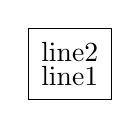
\begin{tikzpicture} [x=1em, y=1ex]
          \draw (0,0) rectangle (3,6);
          \draw (1.5,2) node {line1};
          \draw (1.5,4) node {line2};
        \end{tikzpicture}

      \end{center}
    \end{narrowcolumn}

    \begin{narrowcolumn}
      \begin{center}
        workspace
        \vspace{2ex}

        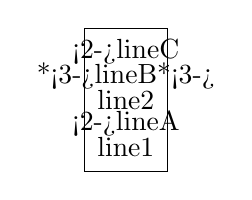
\begin{tikzpicture} [x=1em, y=1ex]
          \draw (0,0) rectangle (3,12);
          \draw (1.5,2) node {line1};
          \draw (1.5,4) node {\alert<2->{lineA}};
          \draw (1.5,6) node {line2};
          \draw (1.5,8) node {\onslide*<3->{\color{blue}}lineB\onslide*<3->{\color{black}}};
          \draw (1.5,10) node {\alert<2->{lineC}};
        \end{tikzpicture}

      \end{center}
    \end{narrowcolumn}

    \begin{narrowcolumn}
      \onslide*<5-8>{

        \code{
          diff {\dhyphen}git a/a b/a

          ...

          +lineC

          \onslide*<-6>{+lineB}

          ~line2

          +lineA

          ~line1

        }
      }

      \onslide*<11->{
      \begin{center}
        cached
        \vspace{2ex}

        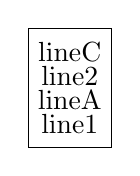
\begin{tikzpicture} [x=1em, y=1ex]
          \draw (0,0) rectangle (3,10);
          \draw (1.5,2) node {line1};
          \draw (1.5,4) node {lineA};
          \draw (1.5,6) node {line2};
          \draw (1.5,8) node {lineC};
        \end{tikzpicture}

      \end{center}

      }
    \end{narrowcolumn}

  \end{columns}
  \vspace{2ex}

  \onslide*<1>{
    調子に乗って、一度に一つのファイルを

    更新しすぎた

    2個の commit に分けたい
  }
  \onslide*<2-3>{
    \alert{この行だけ}次の commit で追加したい
    \vspace{2ex}

    \onslide*<3->{
      \color{blue}この行\color{black}はまた後で commit するので

      workspace で削除したくない
    }
  }
  \onslide*<4>{\$ git add -e \textit{path}}
  \onslide*<5>{エディタでパッチ編集画面が開く}
  \onslide*<6-7>{+lineB の行を消す}
  \onslide*<8-9>{エディタ終了}
  \onslide*<10-11>{
    HEAD のファイルに、

    先ほど編集したパッチを適用した物が

    cached に追加される
  }
  \onslide*<12>{
    この状態で commit すれば、

    workspace の更新を repository に部分適用可能
  }

  \onslide*<13>{
    commit の大きさは程度の問題であり、色々な方針が有ると思うが

    個人的には小さい commit 大好き
  }

  \onslide*<14>{小さい commit は小さい add に宿る}
\end{frame}


\section{未 commit の作業を一時中断する}
% Copyright 2014 Yoshida Shin
% 
% This is part of "Git Second Step."
% 
% This program is free software: you can redistribute it and/or modify
%     it under the terms of the GNU General Public License as published by
%     the Free Software Foundation, either version 3 of the License, or
%     (at your option) any later version.
% 
%     This program is distributed in the hope that it will be useful,
%     but WITHOUT ANY WARRANTY; without even the implied warranty of
%     MERCHANTABILITY or FITNESS FOR A PARTICULAR PURPOSE.  See the
%     GNU General Public License for more details.
% 
%     You should have received a copy of the GNU General Public License
%     along with this program.  If not, see <http://www.gnu.org/licenses/>.

\begin{frame}{}{}
  未 commit の作業を一時中断する
\end{frame}

\begin{frame}[t]{未 commit の作業を一時中断する}{}

  \onslide*<1-2>{
    rebase や cherry-pick は便利だが、

    workspace と cached が clean な時しか実行不可

    (git status で差分が出てきて駄目)

    checkout や merge も clean な状況で行った方が安全

    \vspace{4ex}

    \onslide<2->{
      未 commit のファイルがある状態で

      rebase や cherry-pick を行うには

      どうしたら良いか?
    }
  }

  \onslide*<3-8>{
    \begin{enumerate}
    \item 未 commit のファイルを退避
      \onslide<4->{\item git reset {\dhyphen}hard 実行}
      \onslide<5->{\item rebase や cherry-pick 実行}
      \onslide<6->{\item 退避させたファイルを戻す}
    \end{enumerate}
    \vspace{4ex}

    \onslide<7->{手作業が面倒なので、自動化したい}

    \onslide<8->{そこで stash}
  }

  \onslide*<9-10>{
    \$ git stash
    \vspace{2ex}

    workspace と cached の変更をスタックし

    clean にする
    \vspace{4ex}

    \onslide<10>{
      \$ git stash pop
      \vspace{2ex}

      スタックから workspace と cached の変更を取り出し

      適用する
    }
  }

  \onslide*<11-15>{
    未 commit のファイルがある状態で rebase や cherry-pick を行う

    (stash 使用バージョン)
    \vspace{2ex}

    \onslide<12->{
      \begin{enumerate}
      \item \$ git stash
        \onslide<13->{\item rebase や cherry-pick 実行}
        \onslide<14->{\item \$ git stash pop}
      \end{enumerate}
      \vspace{2ex}

      \onslide<15->{merge や checckout で使っても便利}
    }
  }

  \onslide*<16>{
    ちなみに、
    \vspace{2ex}

    \$ git config {\dhyphen}global rebase.autostash true
    \vspace{2ex}

    とすると、
    \vspace{4ex}

    git rebase と実行するだけで
    \vspace{2ex}

    stash $\rightarrow$ rebase $\rightarrow$ stash pop
    \vspace{2ex}

    を実行してくれるようになる
  }

  \onslide*<17->{
    補足
    \vspace{2ex}

    stash は複数の変更をスタック、保存可能
    \vspace{2ex}

    stash した branch とは別の branch で pop する事も可能
    \vspace{2ex}

    でも、やり過ぎるとかえって頭が混乱するので程々に

    (stash pop で衝突とかすると、泣きたくなります)
    \vspace{2ex}

    複雑になる場合は、一時 branch 作った方が楽かも
  }
\end{frame}


\section{迷子になったら}
% Copyright 2014 Yoshida Shin
% 
% This is part of "Git Second Step."
% 
% This program is free software: you can redistribute it and/or modify
%     it under the terms of the GNU General Public License as published by
%     the Free Software Foundation, either version 3 of the License, or
%     (at your option) any later version.
% 
%     This program is distributed in the hope that it will be useful,
%     but WITHOUT ANY WARRANTY; without even the implied warranty of
%     MERCHANTABILITY or FITNESS FOR A PARTICULAR PURPOSE.  See the
%     GNU General Public License for more details.
% 
%     You should have received a copy of the GNU General Public License
%     along with this program.  If not, see <http://www.gnu.org/licenses/>.

\begin{frame}{}{}
  迷子になったら
\end{frame}

\begin{frame}[t]{迷子になったら}{}

  \onslide*<1-5>{
    git を使っていると、時々迷子になる
    \vspace{4ex}

    \onslide<2->{
      \begin{itemize}
      \item 不要な git reset したけど、よく考えると必要
        \onslide<3->{\item 消してはいけない branch を消してしまった}
        \onslide<4->{\item さっきの rebase をきり戻したい}
        \onslide*<5>{\item 単純なコマンドミス}
      \end{itemize}
    }

  }

  \onslide*<6-8>{
    git では branch や HEAD は

    あくまでリンクもどき
    \vspace{4ex}

    \onslide<7->{
      何をしても、commit 自体はしばらく残る
      \vspace{2ex}

      \onslide<8->{
        commit のハッシュ値さえ分かれば

        いつでも checkout できるし、

        branch も作れる
      }
    }

  }

  \onslide*<9->{
    直近で動いてきた HEAD の履歴を追う
    \vspace{2ex}

    \onslide<10->{
      \$ git reflog
      \vspace{2ex}

      \onslide<11->{
        \code{
          e52e284 HEAD@\{0\}: cherry-pick: G

          11c7ef8 HEAD@\{1\}: reset: moving to 11c7

          01951fe HEAD@\{2\}: cherry-pick: H

          11c7ef8 HEAD@\{3\}: checkout: moving from devel to master

          52f921f HEAD@\{4\}: checkout: moving from master to devel

          11c7ef8 HEAD@\{5\}: commit: J

          ffa3ca9 HEAD@\{6\}: checkout: moving from spike to master

          ...
        }
      }
    }
    \vspace{2ex}

    \onslide<12->{
      このハッシュ値や HEAD@\{n\} のリンクを使用して

      checkout 可能
    }
  }
\end{frame}


\section{git の入れ子管理}
% Copyright 2014 Yoshida Shin
% 
% This is part of "Git Second Step."
% 
% This program is free software: you can redistribute it and/or modify
%     it under the terms of the GNU General Public License as published by
%     the Free Software Foundation, either version 3 of the License, or
%     (at your option) any later version.
% 
%     This program is distributed in the hope that it will be useful,
%     but WITHOUT ANY WARRANTY; without even the implied warranty of
%     MERCHANTABILITY or FITNESS FOR A PARTICULAR PURPOSE.  See the
%     GNU General Public License for more details.
% 
%     You should have received a copy of the GNU General Public License
%     along with this program.  If not, see <http://www.gnu.org/licenses/>.

\begin{frame}{}{}
  git の入れ子管理
\end{frame}

\begin{frame}[t]{git の入れ子管理}{子 repository の使用}

  \begin{columns}

    \begin{narrowcolumn}
      {\small
        \onslide*<1-5>{repo1}\onslide*<6-20>{\color{blue}repo1\color{black}}\onslide*<21->{\color{green}repo1\color{black}}

        ~~{\vbar}-- libs

        \onslide*<3->{
          ~~{\vbar}~~~~{\vbar}-- \alert<9->{repo2}

          ~~{\vbar}~~~~{\vbar}~~~~{\vbar}-- ...
        }

        ~~{\vbar}~~~~{\vbar}-- ...

        \onslide*<3->{~~{\vbar}-- .gitmodules}

        ~~{\vbar}-- ...
        \vspace{3ex}

        \onslide*<11->{
          \onslide*<-23>{\color{blue}clone\color{black}}\onslide*<24->{\color{green}clone\color{black}}

          ~~{\vbar}-- libs

          ~~{\vbar}~~~~{\vbar}-- \alert<26->{repo2}

          \onslide*<15->{~~{\vbar}~~~~{\vbar}~~~~{\vbar}-- ...}

          ~~{\vbar}~~~~{\vbar}-- ...

          ~~{\vbar}-- .gitmodules

          ~~{\vbar}-- ...
        }
      }
    \end{narrowcolumn}

    \begin{widecolumn}

      \onslide*<1>{
        別 repository の repo2 を

        repo1 の中で入れ子管理する

        (repo1 の submodule にする)
      }

      \onslide*<2-3>{
        \alert{workspace の top ディレクトリ}で
        \vspace{2ex}

        \$ git submodule add \textit{URI} libs/repo2
        \vspace{4ex}

        \onslide<3->{
          repo2 が clone され、

          .gitmodules が作成される
        }
      }

      \onslide*<4-6>{
        .gitmodules を commit すれば

        submodule 化完了
        \vspace{2ex}

        \onslide*<5-6>{
          \$ git add .gitmodules

          \$ git commit
        }
      }

      \onslide*<7-9>{
        repo2 以下のディレクトリで

        何をやっても

        repo1 には影響を与えない

        (repo2 以下のディレクトリでは

        ~repo1 は見えない)
        \vspace{2ex}

        \onslide*<8->{
          \$ cd libs/repo2

          \$ touch a

          \$ git add a

          \$ git commit

          \$ git push origin master
        }
        \vspace{2ex}
      }

      \onslide*<10-12>{
        repo1 を clone してみる
        \vspace{2ex}

        \$ git clone repo1 clone
        \vspace{4ex}

        \onslide*<12>{repo2 の中身は空}
      }

      \onslide*<13-16>{
        repo2 を clone するには、別途 submodule update が必要
        \vspace{2ex}

        \onslide*<14->{
          \$ git submodule update {\bslash}

          ~~~~{\dhyphen}init {\dhyphen}recursive

          (全 submodule を clone)
          \vspace{1ex}

          \onslide*<16->{
            {\dhyphen}init

            初めて update する

            submodule がある時に必要
            \vspace{2ex}

            {\dhyphen}recursive

            repo2 がさらに別の submodule を

            管理している場合に必要
          }
        }
      }

      \onslide*<17-18>{
        でも、repo2 の HEAD が古い commit を指している
        \vspace{2ex}

        \onslide*<18>{
          これは、repo1 が submodule の

          バージョンまで管理しているから

          (repo1 で commit した時点の

          ~repo2 の commit へ

          ~checkout している)
        }
        \vspace{2ex}
      }
      \onslide*<19-21>{
        repo2 のバージョンを上げるには、

        repo1 で repo2 の新しいバージョンを commit
        \vspace{2ex}

        \onslide*<20->{
          \$ git add libs/repo2

          \$ git commit

          \$ git push origin master
        }
      }

      \onslide*<22->{
        clone を更新して

        再度 submodule update を行えば

        clone でも repo2 の HEAD が

        切り替わる
        \vspace{2ex}

        \onslide*<23->{
          \$ git fetch {\dhyphen}all -p

          \$ git merge remotes/origin/master

          \onslide*<25->{
            \$ git submodule update {\dhyphen}recursive
            \vspace{2ex}

            (初めて submodule update する

            ~repository は無いので

            ~{\dhyphen}init は不要)
          }
        }
      }
    \end{widecolumn}

  \end{columns}
\end{frame}


% Copyright 2014 Yoshida Shin
% 
% This is part of "Git Second Step."
% 
% This program is free software: you can redistribute it and/or modify
%     it under the terms of the GNU General Public License as published by
%     the Free Software Foundation, either version 3 of the License, or
%     (at your option) any later version.
% 
%     This program is distributed in the hope that it will be useful,
%     but WITHOUT ANY WARRANTY; without even the implied warranty of
%     MERCHANTABILITY or FITNESS FOR A PARTICULAR PURPOSE.  See the
%     GNU General Public License for more details.
% 
%     You should have received a copy of the GNU General Public License
%     along with this program.  If not, see <http://www.gnu.org/licenses/>.

\begin{frame}[t]{git の入れ子管理}{repository の分離}
  git submodule が他 repository を特定ディレクトリに

  対応させるコマンドなら、
  \vspace{2ex}

  特定ディレクトリを独立した repository に

  変換するコマンドは

  git filter-branch
\end{frame}


\begin{frame}[t]{git の入れ子管理}{repository の分離}

  workspace のトップディレクトリで
  \vspace{2ex}

  \$ git filter-branch {\dhyphen}subdirectory-filter {\bslash}
  ~~~~\textit{path\_to\_the\_directory} {\dhyphen} {\dhyphen}all
  \vspace{4ex}

  \onslide*<2->{
    reflog も新しくなるので注意

    (reflog で過去の commit を探して切り戻す事は不可能)
  }
  \vspace{2ex}

  \onslide*<3->{tag も残るが、中身は変更される}
  \vspace{2ex}

  \onslide*<3->{
    ただし、filter-branch 実行前の branch だけなら

    .git/refs/original/refs/head 以下のテキストファイルに

    ハッシュ値が記載

    そこから復旧可能
  }
\end{frame}

\begin{frame}[t]{git の入れ子管理}{}
  ここでは紹介しきれていないが

  submodule も filter-branch も癖が有るコマンドなので

  要注意
  \vspace{4ex}

  実行する前に man を良く確認し、

  バックアップを取ってから

  実行する事を推奨
  \vspace{4ex}

  でも、repository を細かく管理できるのは

  それを補ってあまり有る利便性(だと思う)
\end{frame}


\section{最後に}
\include{conf}

\end{document}
